\subsection{mID Application}

For this component of the system we will be using \textbf{Threat Modelling}, \textbf{focusing on Assets}. We decided that this approach is the best due to the overall state of the system, specially of this component, that is not yet finished.
Alongside this strategy, we are going to use the \textbf{STRIDE} approach complemented with a \textbf{Data Flow Diagram}.

\subsubsection{Focusing on Assets}

When we are Focusing on Assets while searching for potential threats in our system, it is important to think about 3 topics: \textbf{Things attackers want}, \textbf{Things you want to protect}, and \textbf{Stepping stones to either of these.} Considering our mID Application, we answered these topics:

\textbf{Things attackers want}
\begin{itemize}
  \item Steal personal information (Identity Theft for example)
  \item Disrupt/Sabotage service
  \item Change personal information
\end{itemize}

\textbf{Things you want to protect}
\begin{itemize}
  \item Personal Information
  \item Personal Information(data) integrity
  \item Service Reliability/Trustworthiness 
\end{itemize}

\textbf{Stepping stones to either of these}
\begin{itemize}
  \item Encrypt local data
  \item Use secure authentication
  \item Unique and Secure Identifiers for all entities
  \item Safe and Unbreakable logging (for auditing)
\end{itemize}

\subsubsection{System Modelling}

The best way to understand what can go wrong with the mID Application is to understand what it does. To do so, we will be using a \textbf{Data Flow Diagram} to represent this part of the system as well as it's interactions.


\begin{figure}[ht!]
 	\centering
 	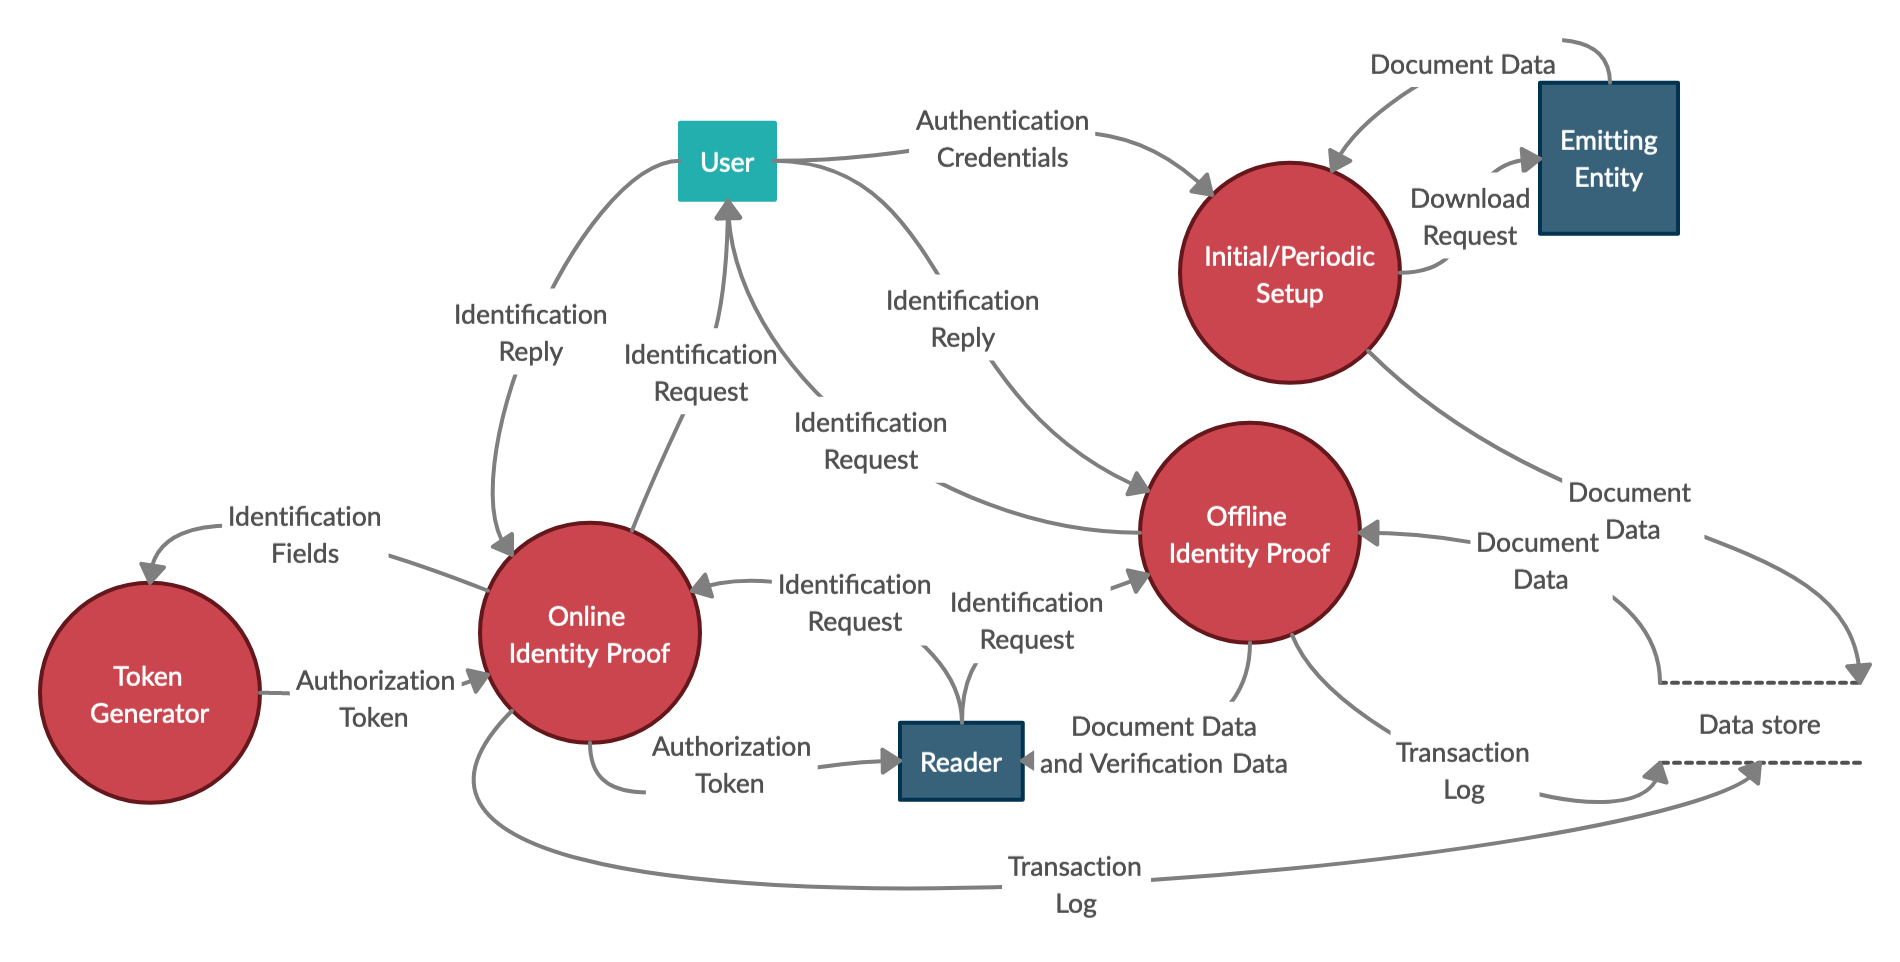
\includegraphics[width=0.94\linewidth]{img/mIDApplicationDFD.png}
 	\caption{mID Application Data Flow Diagram}
 \end{figure}
 
 We represented other elements of the system such as the Reader and Emitting Entity as external entities in order to better represent our communication with them, and, the local storage of the device was represented as a Data store.

\subsubsection{Finding Threats}

With our Data Flow Diagram done, we are now able to analyze it and find threats in a more streamlined way. In order to find the relevant threats, we will be using the STRIDE methodology:

\subsubsection{STRIDE}

\textbf{Spoofing}
\begin{itemize}
    \item The lack of User authentication may lead to an attacker posing as someone being able to download their personal data. This can be fixed by using a secure authentication system, such as \textbf{Two Factor Authentication}. The integration of this service is highly recommended.
    
    \item The communication with the backend without any kind of authentication allows an attacker being able to pose as an Emitting Entity. A good idea would be to implement a \textbf{Public Key Infrastructure} in our system. A PKI is a infrastructure that allow to identify users in a system. The idea is to have one or more trusted parties digitally sign documents certifying that a particular cryptographic key belongs to a particular user or device. The key can then be used as an identity for the user in digital networks.\cite{pki}
    
    \item The communication with the Reader is also vulnerable to spoofing. An attacker could pose as an trusted reader and start the connection process with a user without the user knowing that he is given his information to an attacker and not a trusted reader. This could be also be prevented with the use of a PKI\cite{pki} in our system. This way, the application has the means to check the signature of the reader.
\end{itemize}

\textbf{Tampering}
\begin{itemize}
    \item The local storage of the device has sensitive information, which is a target to attackers. These can be external attackers or even the user of the application. An attacker may, for example,  try to alter information stored. Encrypting this local storage can limit these actions, but, it would also be useful to have a PKI\cite{pki} and use it to sign the information that is stored. With this, we have a way of knowing if a record has been tampered, improving our systems integrity and the authenticity of the information stored.
    \item The fact of some communication being made over the internet leaves the possibility of an attacker tampering our system. It would be a good idea to use secure communication channels for all communications over the Internet. This could be achieved using, for example, \textbf{TLS}. TLS stands for \textbf{Transport Layer Security} and it can be used to encrypt the communication between web applications and servers, emails, messaging, and more.\cite{tls} Between the user and the reader we have two choices: focusing on making the channels secure or encrypting the message. Since we have different kinds of channels, it would be a good idea to focus on \textbf{encrypting the message}, managing to have a solution that works on all channels. On top of the message encryption we could also \textbf{sign the message} with the help of our PKI, allowing us to mitigate this problem.
\end{itemize}

\textbf{Repudiation}
\begin{itemize}
    \item At the moment, we have no way of guaranteeing that a entity is who it claims to be. This is a serious threat to our system that also could be resolved with the addition of a Public Key Infrastructure.\cite{pki}
    \item The lack of certain fields in a transaction may lead to the possibility of an attacker forging one. In order to avoid that, all transaction logs should contain an unique identification tag and information such as the date in which the transaction occurred. It should also be implemented a system to monitor alterations of these logs.
\end{itemize}

\textbf{Information Disclosure}
\begin{itemize}
    \item The local storage containing logs and personal information is vulnerable to an attacker who may try to access that information. This situation could be mitigated by encrypting the local storage, preventing unwanted accesses.
    \item The communication with the emitting entity is not protected, and, vulnerable to being listened to by an attacker that can collect user information. By using TLS\cite{tls} and HTTPS this problem could be mitigated.
    \item The connection process with the reader is done using three different technologies, BLE, NFC and WiFi-Aware. All of these technologies are vulnerable to being listened to by an attacker. As seen before, a good solution would be to encrypt and sign(using our PKI) all the messages sent.
    \item The communication with the reader also lacks protection, leaving the door open to an attacker reading information such as the Authorization Token or personal information. This could the same way as on the connection process, by encrypting messages and signing them. 
    \item The generated Authorization Token has no guarantee that after being sent to the reader it will only be used once. A good solution for this would be the implementation of a \textbf{TTL}(Time To Live) for the token. With this, for example, after a certain time, the token would be rendered useless.
\end{itemize}

\textbf{Denial of Service}
\begin{itemize}
    \item When receiving or updating information from the emitting entity, there is no verification if the incoming data is in fact from whom it claims to be. By not checking this, an attacker could be posing as an emitting entity and try to flood the application with fake data filling the local storage of the device. This could be solved using a PKI\cite{pki}, discarding all packets which are not of interest.
    \item When receiving data, there is no verification if the data is coming from whom we think it does. This could be exploited by an attacker trying to flood the user with incoming data. By filtering the incoming information using a PKI\cite{pki} we could use the signature of the data to decide if we want to discard it, and thus decrease the odds of flooding.
\end{itemize}

\textbf{Elevation of Privilege}
\begin{itemize}
    \item The local storage on the device is vulnerable to an attacker modifying bits on disk in order to run unauthorized commands. This could also be solved by encrypting local storage.
    \item The content of incoming data is not being validated which is a problem. There should be implemented an module to validate incoming data to ensure that there is no malicious code hidden. An attacker could, for example, hide malicious code hidden in data fields and run them on the users device.
\end{itemize}

\subsubsection{Risk Analysis}

With the help of the STRIDE methodology we were able to search for vulnerabilities that the mID Application may encounter when in use. Unfortunately, resources are limited and there are vulnerabilities that are more important and should be addressed first. With that in mind, we tried to evaluate what should be implemented/focused on first. For that process of evaluation we tried to make a \textbf{Risk Analysis}, which involves analyzing the probability of something happening with the impact that is could have. We added also the weight of one solution fixing multiple problems.
Given this, and after making the proper analysis, we decided that from the previous solutions we proposed, the ones that should be focused on first are: the implementation of \textbf{Two Factor Authentication}, the addition of a \textbf{Public Key Infrastructure} to the system both for encryption and data signature, and the use of \textbf{Transport Layer Security} and \textbf{HTTPS} in communications. By adding these functionalities to the system, a big part of the listed vulnerabilities could be mitigated.